\documentclass[11pt]{article}

% Packages
\usepackage[utf8]{inputenc}   % For UTF-8 encoding
\usepackage{amsmath, amssymb} % For mathematical symbols
\usepackage{graphicx}         % For including graphics
\usepackage{geometry}         % For adjusting page dimensions
\usepackage{hyperref}         % For hyperlinks
\usepackage{booktabs}         % For nicer tables
\usepackage{float}            % For figure placement

% Page layout
\geometry{a4paper, margin=1in}

% Document Info
\title{Model for U.S. Population Growth}
\author{Yijia Zhou}
\date{\today}

% Begin Document
\begin{document}

\maketitle


\section{Introduction}
Based on the population from 1790 to 2000, I created two different models to interpolate and fit the original data

\section{Methods}
\subsection{Background}
The following data represent the population of the United States from 1790 to 2000 at ten-year intervals.

\begin{table}[H]
    \centering
    \begin{tabular}{ll}
        \toprule
        Year & Population \\
        \midrule
        1790 & 3929000 \\
        1800 & 5308000 \\
        1810 & 7240000 \\
        1820 & 9638000 \\
        1830 & 12866000 \\
        1840 & 17069000 \\
        1850 & 23192000 \\
        1860 & 31443000 \\
        1870 & 38558000 \\
        1880 & 50156000 \\
        1890 & 62948000 \\
        1900 & 75995000 \\
        1910 & 91972000 \\
        1920 & 105711000 \\
        1930 & 122755000 \\
        1940 & 131669000 \\
        1950 & 150697000 \\
        1960 & 179323000 \\
        1970 & 203212000 \\
        1980 & 226505000 \\
        1990 & 248709873 \\
        2000 & 281416000 \\
        \bottomrule
    \end{tabular}
    \caption{Population of the United States (1790-2000)}
\end{table}


\subsection{Interpolating Polynomial}
Based on the original data, I created an Interpolating Polynomial using the Barycentric method provided by scipy.interpolate package. The reason I did not choose other interpolation methods such as numpy.polynomial or scipy.interpolate.lagrange is they either not very stable for more than 20 data points or not exact within. However, this method does not provide coefficients so I have to calculate manually by solving Vandermonde system through np.vander.

Based on this model, the estimation of population is 182,030,352 in 1968, 7,018,575,493 in 1999, and -38,581,055,260,573 in 2020, indicating that this model is not suitable for prediction because the population number is relatively large and we have more than 20 data points.

\begin{table}[H]
    \centering
    \begin{tabular}{ll}
        \toprule
        Degree & Coefficients \\
        \midrule
        21 & 2.12223e-48 \\
        20 & -1.93908e-44 \\
        19 & 3.24190e-41 \\
        18 & 2.46760e-37 \\
        17 & -1.22292e-33 \\
        16 & 1.54154e-30 \\
        15 & 1.75127e-27 \\
        14 & -3.88945e-24 \\
        13 & -6.79099e-21 \\
        12 & 1.25353e-17 \\
        11 & 1.75582e-14 \\
        10 & -6.46085e-12 \\
        9 & -9.32606e-08 \\
        8 & 8.70353e-05 \\
        7 & -3.97644e-01 \\
        6 & 3.73228e+02 \\
        5 & 1.02268e+07 \\
        4 &  -4.59809e+10 \\
        3 & 9.08908e+13 \\
        2 & -9.71533e+16 \\
        1 & 5.51368e+19 \\
        0 & -1.31235e+22 \\
        \bottomrule
    \end{tabular}
    \caption{Barycentric Polynomial coefficients (highest degree first)}
\end{table}


\begin{figure}[H]
    \centering
    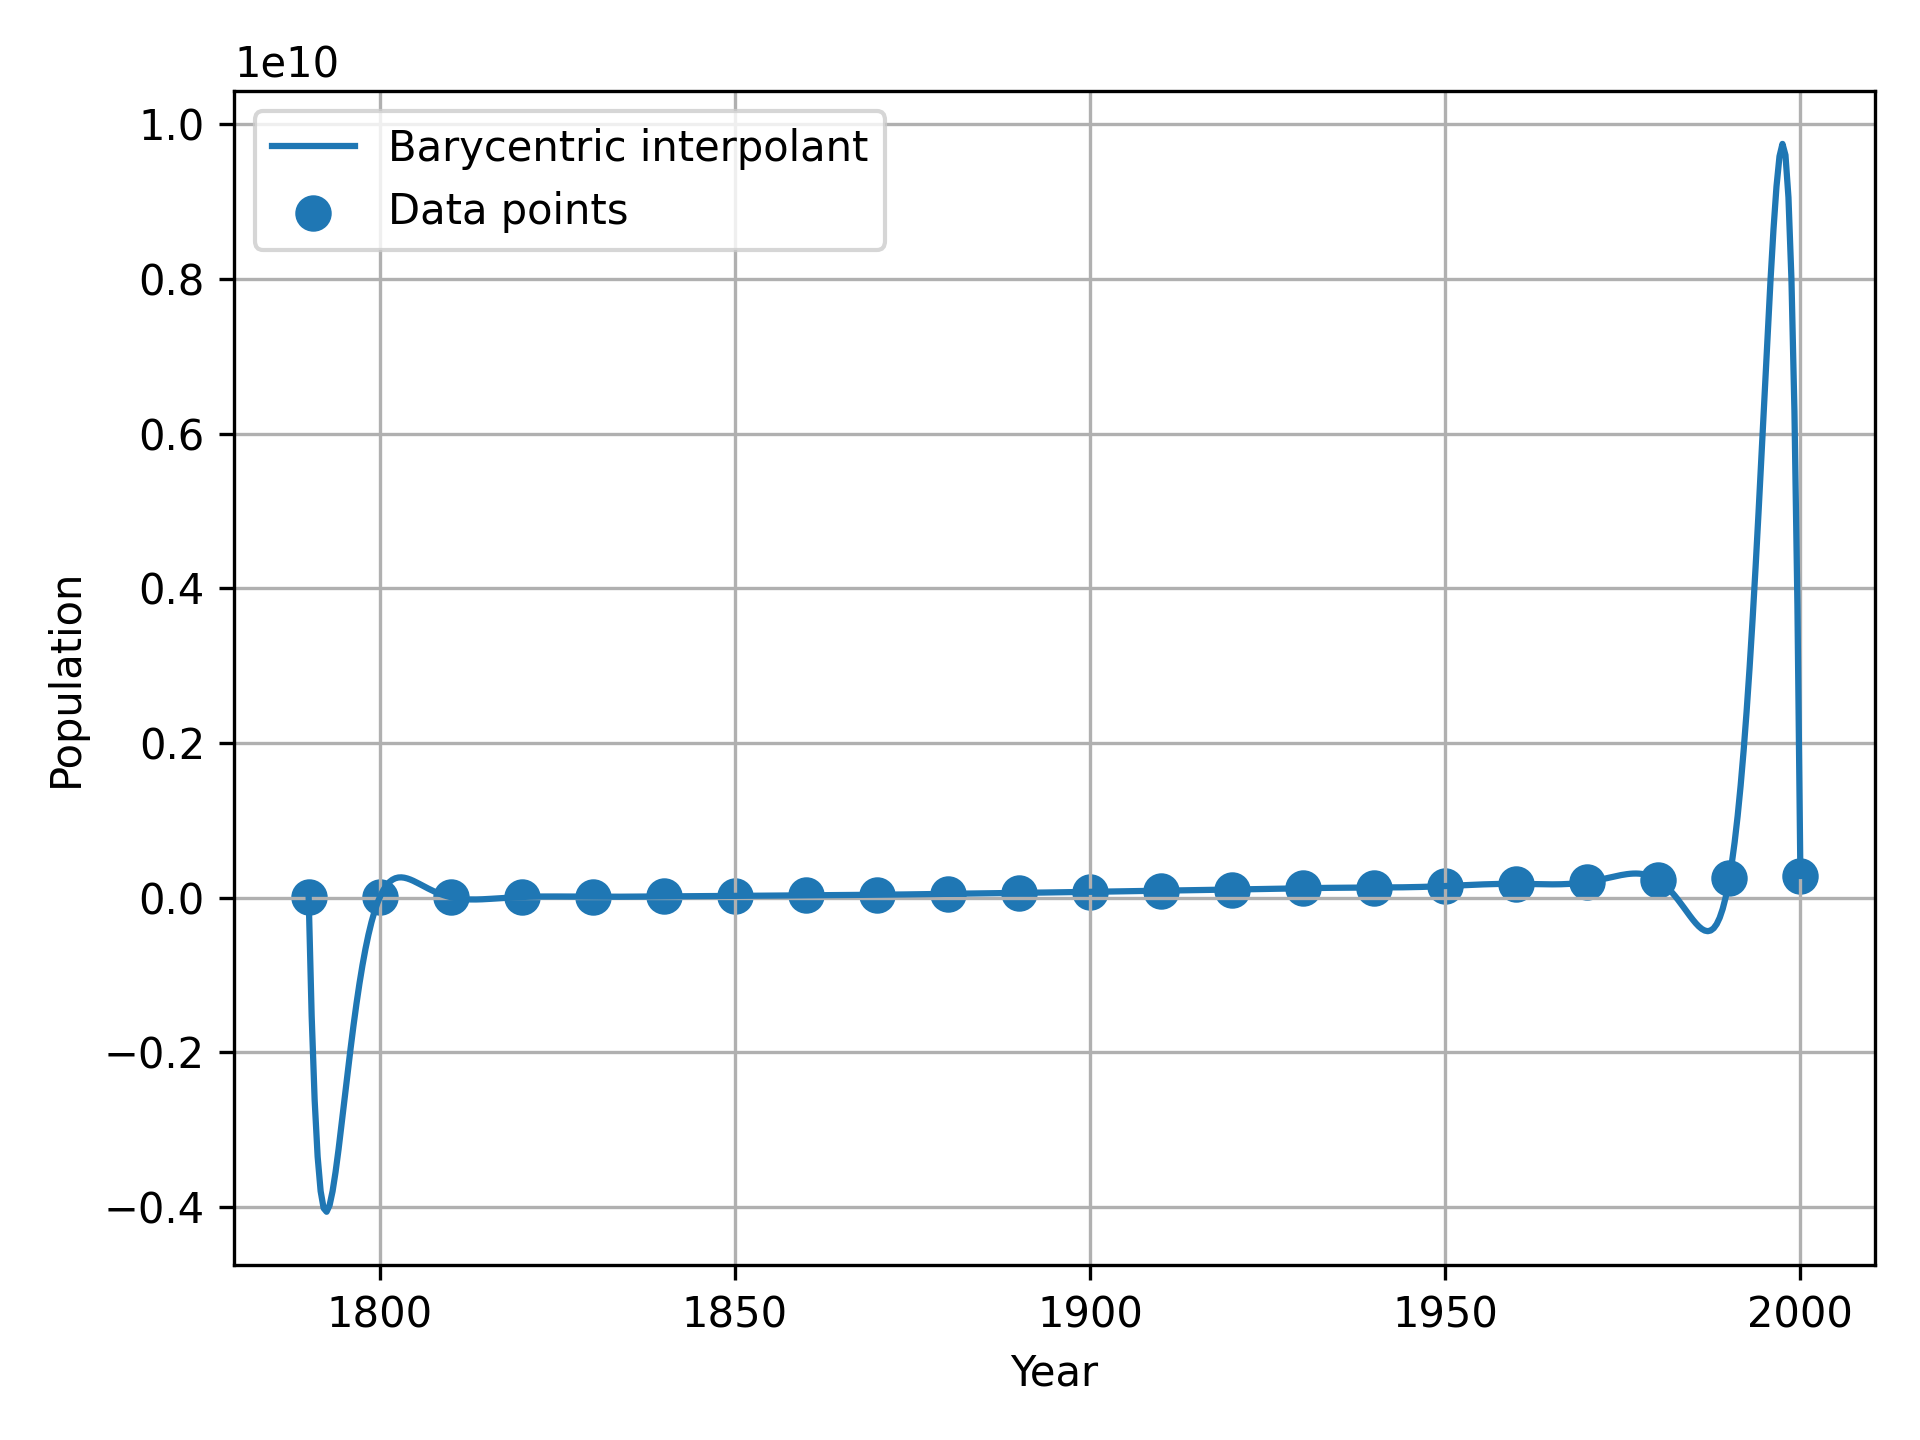
\includegraphics[width=0.5\textwidth]{interpolation_barycentric}
    \caption{Barycentric interpolation}
    \label{interpolation}
\end{figure}


\subsection{Low-order best-fit Polynomial}
Based on the original data, I created a low-order best-fit Polynomial using the numpy.polynomial. The degree of the polynomial is selected based on the largest order than can ensure all divided differences are smaller than the given threshold (0.01 in this case). 

Based on this model, the estimation of population is 195,019,217 in 1968, 277,464,138 in 1999, and 330,262,280 in 2020, which is 331,449,281 based on the United States census. It shows this model performs much better in terms of prediction as the error is about $0.358\%$.
\begin{table}[H]
    \centering
    \begin{tabular}{ll}
        \toprule
        Degree & Coefficients \\
        \midrule
        6 & -2.88489e-05 \\
        5 & 3.28845e-01 \\
        4 &  -1.56131e+03 \\
        3 & 3.95214e+06 \\
        2 & -5.6253e+09 \\
        1 & 4.26879e+12 \\
        0 & -1.31235e+22 \\
        \bottomrule
    \end{tabular}
    \caption{Best fit coefficients (highest degree first)}
\end{table}

\begin{figure}[H]
    \centering
    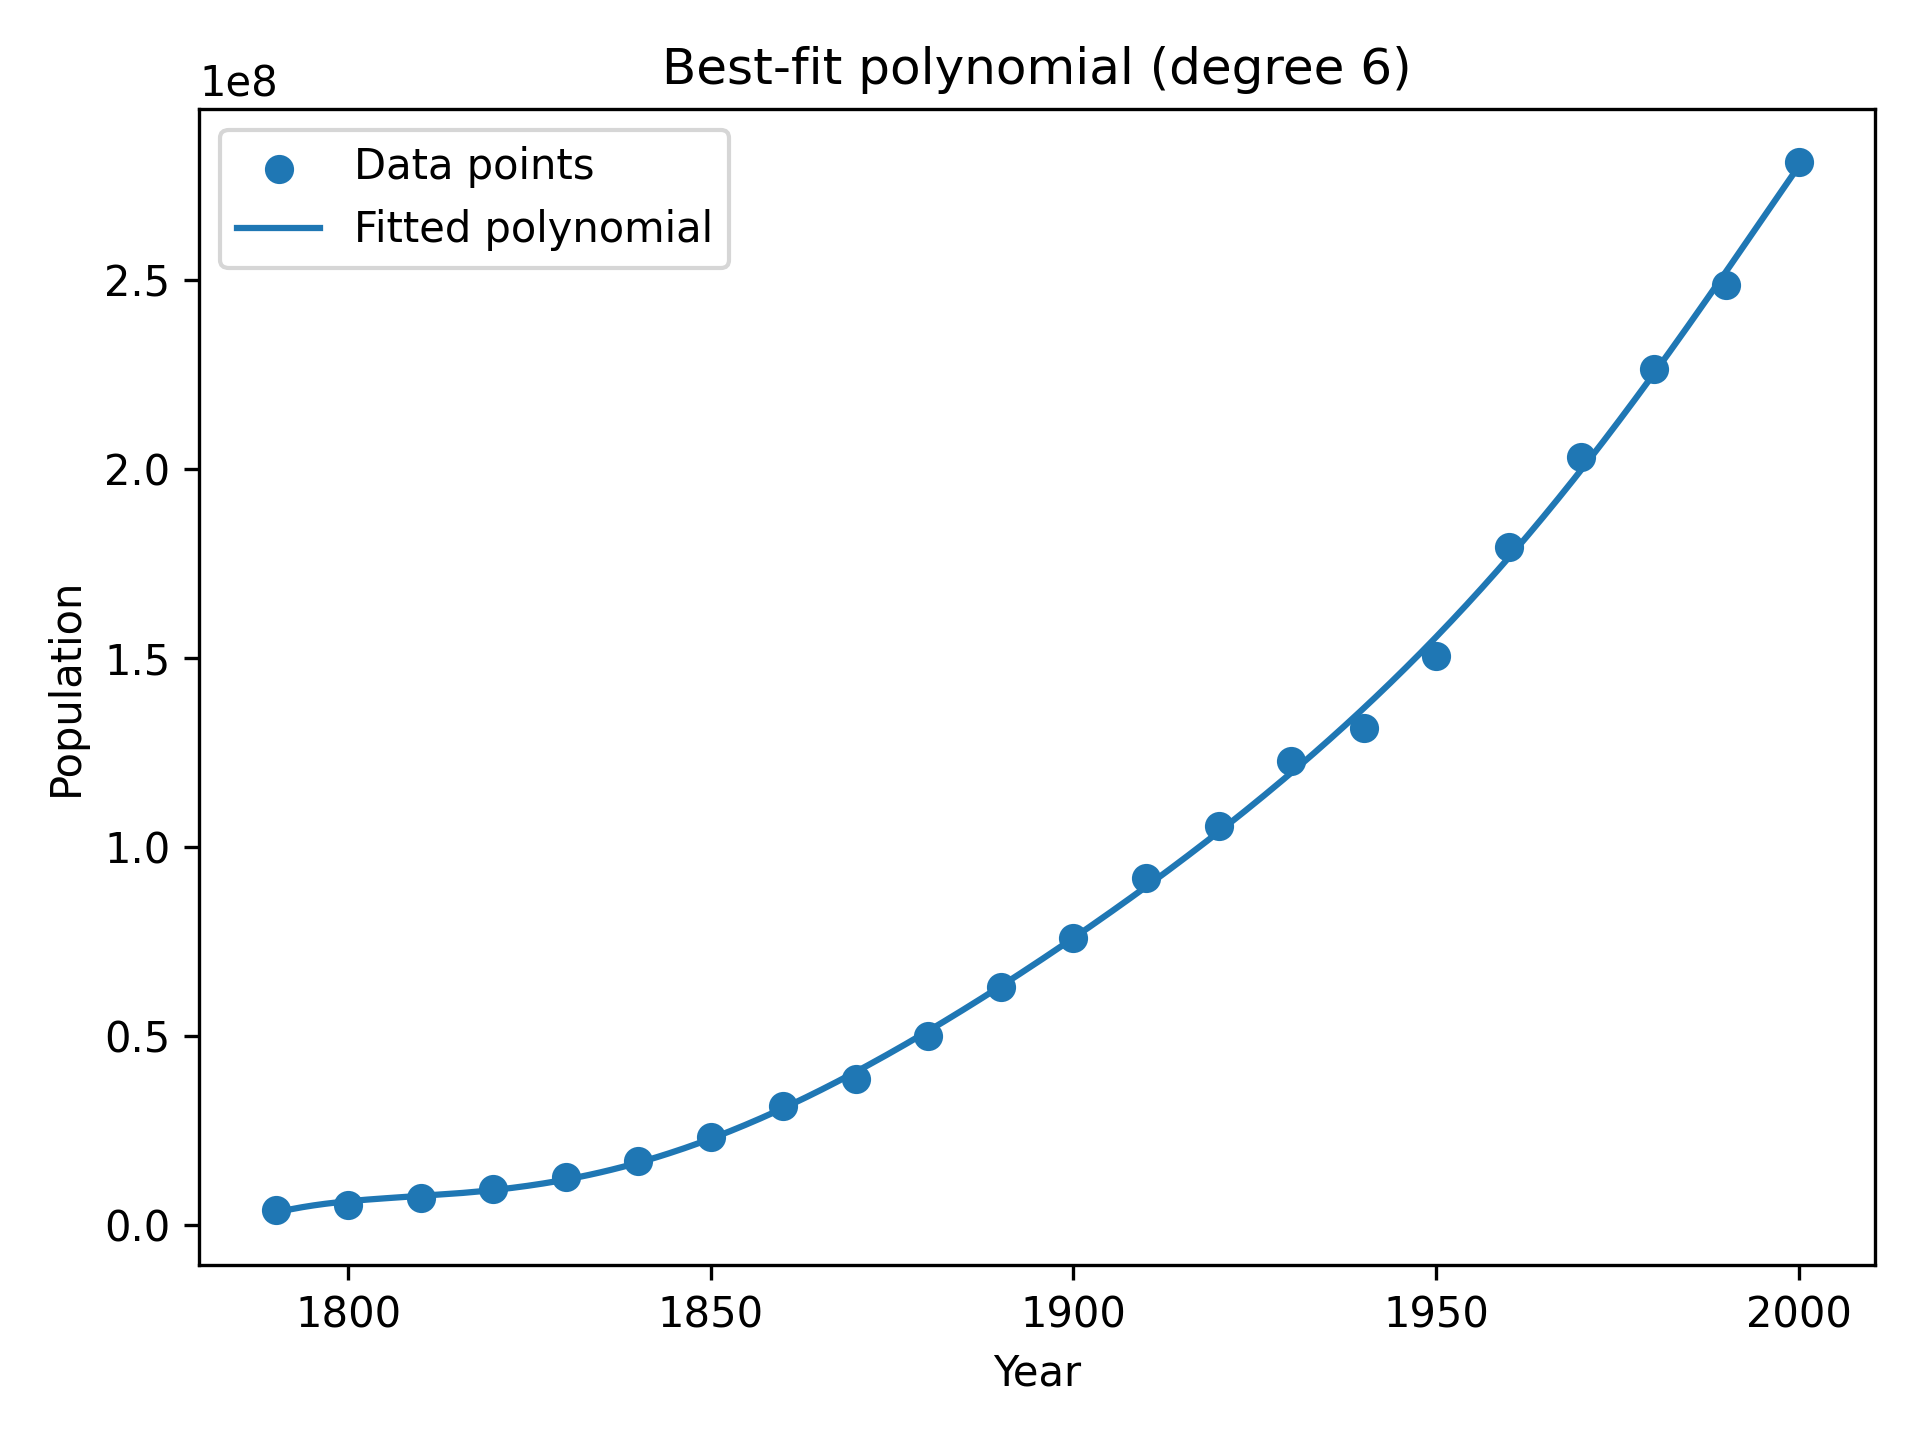
\includegraphics[width=0.5\textwidth]{polynomial_fit}
    \caption{Polynomial fit}
    \label{fit}
\end{figure}

\section{Conclusion}
I created two different models to interpolate and fit the original data. The first model is an Interpolating Polynomial using the Barycentric method provided by scipy.interpolate package. However, this model is not suitable for prediction because the population number is relatively large and we have >20 data points. The second model is a low-order best-fit Polynomial using the numpy.polynomial package. This model performs much better in terms of prediction.


\end{document}